% Foliensatz: "AFu-Kurs nach DJ4UF" von DK0TU, Amateurfunkgruppe der TU Berlin
% Lizenz: CC BY-NC-SA 3.0 de (http://creativecommons.org/licenses/by-nc-sa/3.0/de/)
% Autoren: Sebastian Lange <dl7bst@dk0tu.de>
% Korrekturen: Lars Weiler <dc4lw@drac.de>

\documentclass[aspectratio=169]{beamer}

\usepackage[ngerman]{babel} % deutsche Worttrennung etc.
\usepackage[utf8]{inputenc} % UTF8 Text

\usepackage[super, comma, numbers, square, sort]{natbib}

\usepackage{hyperref}       % Hyperref Package für bessere Referenzen (todo)
\hypersetup{
	colorlinks=false,       %   false: boxed links; true: colored links
    %linkcolor=white,       %   color of internal links (change box color with linkbordercolor)
    citecolor=red,          %   color of links to bibliography
    filecolor=white,        %   color of file links
    urlcolor=blue           %   color of external links
}

\usepackage{multirow}
\usepackage{wasysym}  % Math Symbols like \permil
%\usepackage{colortbl}
%\usepackage{subscript}
%\usepackage{caption}
%\usepackage{setspace}
%\usepackage{xcolor}        % benutze CodeListe

% Footnote
%\usepackage{hanging}
%
%\setbeamertemplate{footnote}{%
%  \hangpara{2em}{1}%
%  \makebox[2em][l]{\insertfootnotemark}\footnotesize\insertfootnotetext\par%
%}


%\usepackage{pgf}
%\usepackage{tikz}
%\usetikzlibrary{arrows,automata}
%\usetikzlibrary{positioning}
%
%\tikzset{
%    state/.style={
%           rectangle,
%           rounded corners,
%           draw=black, very thick,
%           minimum height=2em,
%           minimum width=2pt,
%           inner sep=2pt,
%           text centered,
%           },
%}

%\usepackage{listings}
%\lstset{basicstyle=\small, numberstyle=\tiny, extendedchars=true, numbers=left, numbersep=5pt}
%\lstset{showtabs=false, showspaces=false, showstringspaces=false}
%%\lstset{backgroundcolor=\color{white!75!lightgray}, , frame=single}
%%\lstset{backgroundcolor=\color{white}}
%%\lstset{backgroundcolor=none}
%\lstset{keywordstyle=\color{blue!50!gray},  identifierstyle=\color{black}}
%\lstset{commentstyle=\color{green!50!gray}, stringstyle=\color{red!50!gray}}
%\lstset{language=C, fontadjust=true, tabsize=2, breaklines=true}
%\lstset{backgroundcolor=\color{white!75!lightgray}, caption=\lstname, frame=single}
%\lstset{emphstyle=\color{black}\fbox}
%
%% Keine "Listing:"-Caption
%\captionsetup{labelformat=empty,labelsep=none}
%
%% für mathematische Umgebungen
%\usepackage{amsmath,amsfonts,amssymb}
%
%\lstdefinestyle{Bash}{
%language=Bash,
%frame=single,
%rulecolor=\color{black},
%backgroundcolor=\color{gray!50},
%keywordstyle=\color{black},
%identifierstyle=,
%commentstyle=\color{black},
%stringstyle=\color{magenta!65!white},
%showstringspaces=false,
%basicstyle=\footnotesize\ttfamily\color{black},
%numbers=none,
%breaklines=true,
%captionpos=b
%}

%\usepackage{listings}
%
%\lstdefinestyle{basic}{
%    captionpos=t,%
%    basicstyle=\footnotesize\ttfamily,%
%    numberstyle=\tiny,%
%    numbers=left,%
%    stepnumber=1,%
%    frame=single,%
%    showspaces=false,%
%    showstringspaces=false,%
%    showtabs=false,%
%    %
%    keywordstyle=\color{blue},%
%    identifierstyle=,%
%    commentstyle=\color{gray},%
%    stringstyle=\color{magenta}%
%}



% fließende Boxen haben keinen Abstand
%\fboxsep0mm

% inkludiere Creative Commons Helper
%%%%%%%%%%%%%%%%%%%%%%%%%%%%%%%%%%%%%%%%%%%%%%%%%%%%%%%%%%%%%%%%
%% ccBeamer 0.1, 2007-07-02                                   %%
%% Written by Sebastian Pipping <webmaster@hartwork.org>      %%
%% ---------------------------------------------------------- %%
%% Licensed under Creative Commons Attribution-ShareAlike 3.0 %%
%% http://creativecommons.org/licenses/by-sa/3.0/             %%
%%%%%%%%%%%%%%%%%%%%%%%%%%%%%%%%%%%%%%%%%%%%%%%%%%%%%%%%%%%%%%%%


%% Images
\newcommand{\CcImageBy}[1]{%
	
\includegraphics[scale=#1]{texdata/creative_commons/cc_by_30.pdf}%
}
\newcommand{\CcImageCc}[1]{%
	
\includegraphics[scale=#1]{texdata/creative_commons/cc_cc_30.pdf}%
}
\newcommand{\CcImageDevNations}[1]{%
	
\includegraphics[scale=#1]{texdata/creative_commons/cc_dev_nations_30.pdf}%
}
\newcommand{\CcImageNc}[1]{%
	
\includegraphics[scale=#1]{texdata/creative_commons/cc_nc_30.pdf}%
}
\newcommand{\CcImageNd}[1]{%
	
\includegraphics[scale=#1]{texdata/creative_commons/cc_nd_30.pdf}%
}
\newcommand{\CcImagePd}[1]{%
	
\includegraphics[scale=#1]{texdata/creative_commons/cc_pd_30.pdf}%
}
\newcommand{\CcImageSa}[1]{%
	
\includegraphics[scale=#1]{texdata/creative_commons/cc_sa_30.pdf}%
}
\newcommand{\CcImageSampling}[1]{%
	
\includegraphics[scale=#1]{texdata/creative_commons/cc_sampling_30.pdf}%
}
\newcommand{\CcImageSamplingPlus}[1]{%
	
\includegraphics[scale=#1]{texdata/creative_commons/cc_sampling_plus_30.pdf}%
}


%% Groups
\newcommand{\CcGroupBy}[2]{% zoom, gap
	\CcImageCc{#1}\hspace*{#2}\CcImageBy{#1}%
}
\newcommand{\CcGroupByNc}[2]{% zoom, gap
	\CcImageCc{#1}\hspace*{#2}\CcImageBy{#1}\hspace*{#2}\CcImageNc{#1}%
}
\newcommand{\CcGroupByNcNd}[2]{% zoom, gap
	\CcImageCc{#1}\hspace*{#2}\CcImageBy{#1}\hspace*{#2}\CcImageNc{#1}\hspace*{#2}\CcImageNd{#1}%
}
\newcommand{\CcGroupByNcSa}[2]{% zoom, gap
	\CcImageCc{#1}\hspace*{#2}\CcImageBy{#1}\hspace*{#2}\CcImageNc{#1}\hspace*{#2}\CcImageSa{#1}%
}
\newcommand{\CcGroupByNd}[2]{% zoom, gap
	\CcImageCc{#1}\hspace*{#2}\CcImageBy{#1}\hspace*{#2}\CcImageNd{#1}%
}
\newcommand{\CcGroupBySa}[2]{% zoom, gap
	\CcImageCc{#1}\hspace*{#2}\CcImageBy{#1}\hspace*{#2}\CcImageSa{#1}%
}
\newcommand{\CcGroupDevNations}[2]{% zoom, gap
	\CcImageCc{#1}\hspace*{#2}\CcImageDevNations{#1}%
}
\newcommand{\CcGroupNcSampling}[2]{% zoom, gap
	\CcImageCc{#1}\hspace*{#2}\CcImageNc{#1}\hspace*{#2}\CcImageSampling{#1}%
}
\newcommand{\CcGroupPd}[1]{% zoom
	\CcImagePd{#1}%
}
\newcommand{\CcGroupSampling}[1]{% zoom
	\CcImageSampling{#1}%
}
\newcommand{\CcGroupSamplingPlus}[1]{% zoom
	\CcImageSamplingPlus{#1}%
}


%% Text
\newcommand{\CcLongnameBy}{Attribution}
\newcommand{\CcLongnameByNc}{Attribution-NonCommercial}
\newcommand{\CcLongnameByNcNd}{Attribution-NoDerivs}
\newcommand{\CcLongnameByNcSa}{Attribution-NonCommercial-ShareAlike}
\newcommand{\CcLongnameByNd}{Attribution-NoDerivs}
\newcommand{\CcLongnameBySa}{Attribution-ShareAlike}

\newcommand{\CcNote}[1]{% longname
	This work is licensed under the \textit{Creative Commons #1 3.0 License}.%
}


% generelles Thema auswählen
\usetheme{Goettingen} %Berlin spart ohne Sidebar allerdings angenehm Platz
% AnnArbor | Antibes | Bergen | Berkeley | Berlin | Boadilla | boxes | CambridgeUS | Copenhagen | Darmstadt | default | Dresden | Frankfurt | Goettingen | Hannover | Ilmenau | JuanLesPins | Luebeck | Madrid | Malmoe | Marburg | Montpellier | PaloAlto | Pittsburgh | Rochester | Singapore | Szeged | Warsaw

% Farben wählen
\usecolortheme{beetle}
% beaver | beetle | crane | default | dolphin | dove | fly | lily | orchid | rose | seagull | seahorse | sidebartab | structure | whale | wolverine

% Setze alle Farben auf Grau und Weiß
%\definecolor{craneorange}{RGB}{64,64,64}
%\definecolor{craneblue}{RGB}{255,255,255}

% Schriftart wählen
\usefonttheme{default}
% default | professionalfonts | serif | structurebold | structureitalicserif | structuresmallcapsserif

% Innere Themen(Kopf-, Fuß-, Sidebar usw)
%\useinnertheme{default}
\useinnertheme{circles}
% default | inmargin | rectangles | rounded | circles

% Äußere Themen (Anordnung der inneren, grenzen der Folien etc.)
\useoutertheme{infolines}
% default | infolines | miniframes | shadow | sidebar | smoothbars | smoothtree | split | tree

% Deaktiviere Navigations-Symbole ({} -> leer)
\setbeamertemplate{navigation symbols}{}
%\setbeamertemplate{navigation symbols}{\large \ifnum \insertframenumber <10 0\fi\insertframenumber/\inserttotalframenumber\vspace*{0.2ex}}

% Zeige ein Hintergrundbild
\setbeamertemplate{background canvas}{
        \hspace*{-2.0cm}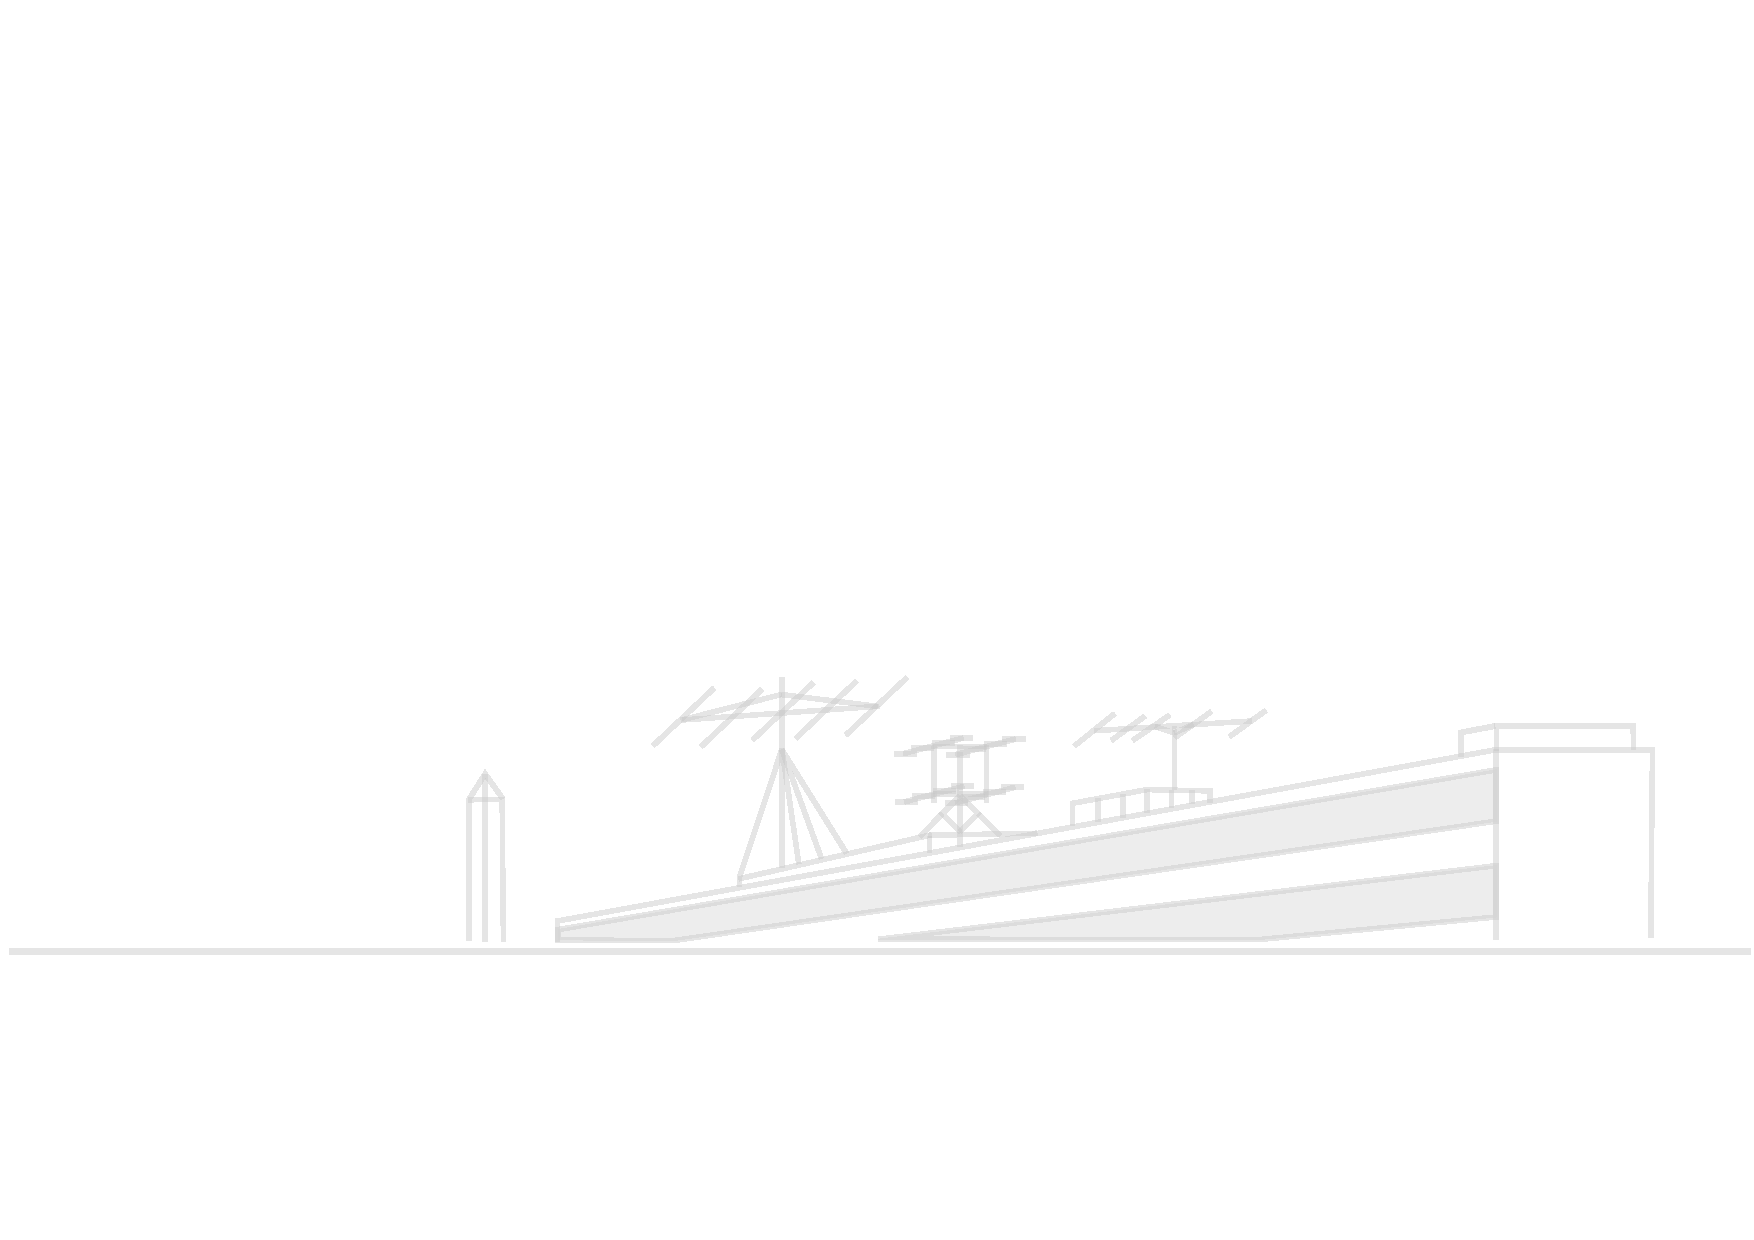
\includegraphics[width=17.8cm]{texdata/dk0tu_rooftop_background.pdf}
}

% Foliennummer einfügen
\setbeamertemplate{footline}[frame number]
%\setbeamertemplate{footline}{}

% Ändere das Zeichen vor jedem item
%\setbeamertemplate{itemize item}{\color{craneorange}$\blacktriangleright$}
%\setbeamertemplate{itemize subitem}{\color{craneorange}$\triangleright$}
%\setbeamertemplate{itemize subsubitem}{\color{craneorange}$\blacktriangleright$}

% Ändert die Blöcke 
\setbeamertemplate{blocks}[rounded][shadow=true]
% default | rounded [shadow=true|false]

%
% Eigene Kommandos
%

% Hack to get natbib and beamer working together. "The beamer user guide suggests
% that only the manual bibliography entry approach is supported"
% on some system it works out of the box, sometimes you need the hack :-(
% so check it --dl7bst
\ifdefined\newblock
    \relax
\else
    \newcommand{\newblock}{}
\fi

% \includedia command to generate png out of a dia file
% NEEDS installed dia and pdflatex option --shell-escape
\newcommand{\includedia}[1]{
    \immediate\write18{/usr/bin/dia #1.dia -e #1_diatmp.png -t png}
}

% RICHIG GROSSER FONT!
\newfont{\bigfont}{cmr10 at 144pt}
\newfont{\smallfont}{cmr10 at 8pt}

% Römische Ziffern
\makeatletter
\newcommand{\rmnum}[1]{\romannumeral #1}
\newcommand{\Rmnum}[1]{\expandafter\@slowromancap\romannumeral #1@}
\makeatother

% Schwarze Überschrift
%\setbeamercolor{frametitle}{fg=black}
%\setbeamercolor{title}{fg=black}

% Item- und Box-Farben
\definecolor{deepBlue}{HTML}{000066}
\setbeamercolor{itemize item}{fg=deepBlue}
\setbeamercolor{itemize subitem}{fg=deepBlue}
\setbeamercolor{description item}{fg=deepBlue}
\setbeamercolor{block title}{fg=deepBlue!100, bg=blue!15}
\setbeamercolor{block body}{fg=black, bg=blue!5}
\setbeamercolor{block title alerted}{fg=deepBlue, bg=red!75}
\setbeamercolor{block body alerted}{fg=black, bg=red!15}
\setbeamercolor*{block title example}{fg=blue!50, bg=blue!10}
\setbeamercolor*{block body example}{fg= blue, bg=blue!5}

%\setbeamercolor{section in head/foot}{parent=palette primary}
%\setbeamercolor{subsection in head/foot}{parent=palette secondary}
%\setbeamercolor{sidebar}{fg=darkblue,bg=yellow!90!orange}
%\setbeamercolor{title in sidebar}{fg=darkblue}
%\setbeamercolor{author in sidebar}{fg=darkblue}
%\setbeamercolor{section in sidebar}{fg=darkblue!10!black}
%\setbeamercolor{subsection in sidebar}{fg=darkblue!50!black}

% Titlepage Infos
\title{AFu-Kurs nach DJ4UF}
\author[DKØTU]{DKØTU\\ \footnotesize{Amateurfunkgruppe der TU Berlin}}
\institute[DKØTU]{\url{http://www.dk0tu.de} }

% PDF-Eigenschaften
\subject{DK0TU-Amateurfunkkurs nach DJ4UF}
\keywords{Amateurfunk Kurs HAM Radio Course CC-BY-NC-SA OpenSource TU Berlin DK0TU}

\subtitle{Technik Klasse A 18: \\
  Gerätetechnik \\[2em]}
\date{Stand 13.03.2017}
 \begin{document}

\begin{frame}
    \titlepage
    \vfill
    \begin{center}
        \ccbyncsaeu\\
        {\tiny This work is licensed under the \em{Creative Commons Attribution-NonCommercial-ShareAlike 3.0 License}.}\\[0.5ex]
         \tiny Amateurfunkgruppe der Technische Universität Berlin (AfuTUB), DKØTU
         %\includegraphics[scale=0.5]{img/DK0TU_Logo.pdf}
    \end{center}
\end{frame}


\section{Überblick}

\begin{frame}
  \frametitle{Überblick}

  Themen aus dem Kapitel \emph{E15 - Sender- und Empfängertechnik} werden hier
  weiterführend behandelt.

  \bigskip

  % TODO Drake Foto?

  Woraus bestehen Sender und Empfänger und welche Haupteigenschaften fallen
  euch ein?

\end{frame}

\section{Empfindlichkeit}

\begin{frame}
  \frametitle{Wiederholung SNR}

  \begin{center}
    \begin{figure}
      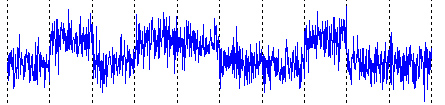
\includegraphics[width=0.8\textwidth,height=.25\textheight,keepaspectratio]{a18/Received_message.jpg}
      \attribcaption{Empfangenes Signal von 0101100100 mit einem SNR von 3dB}{El pak}{https://commons.wikimedia.org/wiki/File:Received_message.jpg}{\ccbysa}
    \end{figure}
  \end{center}

  \begin{center}
    \begin{figure}
      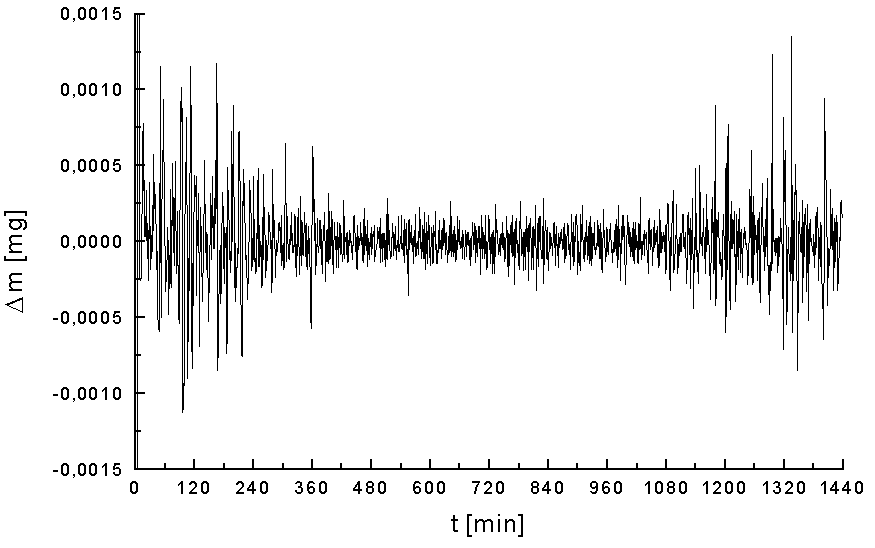
\includegraphics[width=0.8\textwidth,height=.35\textheight,keepaspectratio]{a18/Analyse_thermo_gravimetrique_bruit.png}
      \attribcaption{Aufnahme einer Thermogravimetrischen Analyse mit schlechter Isolierung; nachts ist weniger Rauschen}{Christophe Dang Ngoc Chan (cdang)}{https://commons.wikimedia.org/wiki/File:Analyse_thermo_gravimetrique_bruit.png}{\ccbysa}
    \end{figure}
  \end{center}

\end{frame}

\begin{frame}
  \frametitle{Empfindlichkeit}

  Empfindlichkeit gibt an, wie stark das Eingangssignal sein muss, um über
  dem thermischen Eigenrauschen zu liegen.\\[.5em]

  Einfacher: Fähigkeit des Empfängers, schwache Signale zu empfangen.

  \bigskip

  Wahrnehmungsschwelle des menschlichen Ohrs bei ca. $6 dB$\\
  Sprache ist ab etwa $10 dB$ wahrnehmbar

\end{frame}

\begin{frame}
  \frametitle{Empfindlichkeit}

  \begin{block}{Rauschleistung (Formelsammlung)}
    $P_R = k \cdot T_K \cdot B$\\
    mit $k$: Boltzmann-Konstante, $T_K$: Temperatur in Kelvin, $B$: Bandbreite
  \end{block}

  \bigskip

  \textbf{Die Leistung eines gleichmäßig über einen Frequenzbereich
  verteilten Rauschens ist proportional zur Bandbreite!}

  \bigskip

  \begin{exampleblock}{Wie verhält sich bei sonst gleich bleibenden Bedingungen die
    Rauschleistung nach Umschaltung von SSB auf CW?}
    \only<1>{\vspace{2em}}
    \only<2>{$\cfrac{2,5 kHz}{0,5 kHz} \approx \cfrac{1}{5}$}
  \end{exampleblock}

\end{frame}

\subsection{Rauschzahl}

\begin{frame}
  \frametitle{Rauschzahl}

  Jedes Gerät produziert Eigenrauschen. Die Rauschzahl $F$ (noise figure) ist
  der Faktor, um den die theoretischen Rauschformeln gerätespezifisch
  erweitert werden.

  \bigskip

  Angaben sind als Faktor oder in $dB$ möglich.

  \bigskip

  \begin{exampleblock}{Beispiele}
    $F=1,8 dB \rightarrow$ am Ausgang $1,8dB$ geringeres SNR als am Eingang\\
    $F=2 \rightarrow$ am Ausgang \only<1>{\textbf{?}} \only<2>{$3dB$ geringeres} SNR als am Eingang
  \end{exampleblock}

\end{frame}

\begin{frame}
  \frametitle{Rauschzahl}

  Für Kurzwelle und niedrigere Frequenzen spielt die Rauschzahl keine Rolle,
  da QRN und QRM das SNR bestimmen.

  \bigskip

  Empfindlichkeiten werden bei HF z.B. mit $0,25 \mu V$ Eingangsspannung für
  $S/N=10 dB$ angegeben.

\end{frame}

\begin{frame}
  \frametitle{Rauschzahl}

  VHF/UHF-Vorverstärker möglichst direkt an der Antenne. Warum?\\
  \only<1>{\vspace{2em}}
  \only<2>{Ursache: (Langes) Kabel zwischen Antenne und Empfängereingang
  verschlechtert die Rauschzahl mit seiner Dämpfung}

  \bigskip

  Empfindlichkeit kann auch durch starke HF-Signale auf einer nahen Frequenz
  beeinträchtigt werden $\rightarrow$ Selektivität.

\end{frame}

\subsection{Selektivität}

\begin{frame}
  \frametitle{Selektivität}

  \begin{columns}
    \column{.5\textwidth}
    \begin{center}
      \begin{figure}
        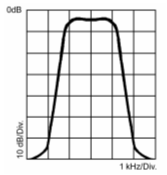
\includegraphics[width=\textwidth,height=.7\textheight,keepaspectratio]{a18/TF410.png}
        \attribcaption{TF410--411}{BNetzA}{https://www.bundesnetzagentur.de/amateurfunk/}{}
      \end{figure}
    \end{center}

    \column{.45\textwidth}

    Fähigkeit, Signale mit steilen Filterflanken zu selektieren. Deshalb auch:
    Trennschärfe.

    \begin{exampleblock}{Grenzbandbreite bei -60 dB? Für welche Signale geeignet?}
      \only<1>{\vspace{1em}}
      \only<2>{4\,kHz, SSB}
    \end{exampleblock}

  \end{columns}

\end{frame}

\begin{frame}
  \frametitle{Selektivität}

  Für einen steilen und schmalen Bandpass eignen sich am besten
  Quarzkristalle.


  \begin{exampleblock}{Welche Filterbandbreiten würdet ihr für J3E, F1B (RTTY Shift 170\,Hz), F3E nutzen?}
    \only<1>{\vspace{3em}}
    \only<2>{
    \begin{description}
      \item[J3E] 2,2\,kHz
      \item[F1B] 500\,Hz
      \item[F3E] 12\,kHz
    \end{description}
    }
  \end{exampleblock}
\end{frame}

\section{HF-Regelung}

\subsection{AGC}

\begin{frame}
  \frametitle{AGC}

  Automatic Gain Control (AGC) sorgt für konstante NF auch bei schwankendem
  HF-Eingang.

  \bigskip

  $\rightarrow$ Bei starkem Eingangssignal wird die Verstärkung der HF- und
  ZF-Stufen reduziert.

\end{frame}

\subsection{Squelch}

\begin{frame}
  \frametitle{Squelch}

  Steuert die ZF- oder NF-Signale, um Grundrauschen auszublenden.

  \bigskip

  Einstellung des Levels etwas über den Rauschen und unterhalb des erwarteten
  Eingangssignals.

\end{frame}

\section[Störungsverm.]{Störungsverminderung}

\begin{frame}
  \frametitle{Störungsverminderung}

  Es werden kurz Beispiele zur Störungsverminderung angerissen.

  \bigskip

  Prüfungsrelevant ist lediglich der Notchfilter.

\end{frame}

\subsection{Passband-Tuning}

\begin{frame}
  \frametitle{Passband-Tuning}

  Durch IF/ZF-Shift wird die Filterkurve soweit verschoben, dass das
  Störsignal ausgeblendet wird.

  \bigskip

  \emph{Beispiel: \href{https://youtu.be/NnhZbAKXm28}{$\Rightarrow$ Passband Tuning vs. IF Shift}}

\end{frame}

\subsection{Bandwidth-Tuning}

\begin{frame}
  \frametitle{Bandwidth-Tuning}

  Übereinanderschieben von steilflankigen Filtern, sodass der
  Durchlassbereich kleiner wird.

  % FIXME Gutes Bild finden oder bauen

  \bigskip

  Wie verhält sich das SNR?
  \only<2>{Proportional zur Bandbreite. Remember?}

\end{frame}

\subsection{Notchfilter}

\begin{frame}
  \frametitle{Notchfilter}

  \begin{columns}
    \column{.5\textwidth}
    \begin{center}
      \begin{figure}
        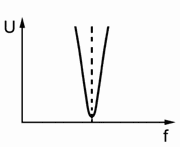
\includegraphics[width=\textwidth,height=.8\textheight,keepaspectratio]{a18/TF326a.png}
        \attribcaption{TF326}{BNetzA}{https://www.bundesnetzagentur.de/amateurfunk/}{}
      \end{figure}
    \end{center}

    \column{.45\textwidth}
    Auch: Kerbfilter mit ``Loch'' im IF-Durchlassbereich zum Ausblenden
    schmalbandiger Störungen.

  \end{columns}


\end{frame}

\subsection{Störbegrenzer/-austaster}

\begin{frame}
  \frametitle{Störbegrenzer/-austaster}

  Störbegrenzer schneidet Spitzenspannungen ab gewissem NF-Pegel ab
  $\rightarrow$ Clipping.

  \bigskip

  Störaustaster regelt bei Störungen ZF oder NF komplett herunter
  $\rightarrow$ Noise Blanker.

  % TODO Zeichnungen?

\end{frame}

\section{Groß"-signal"-festig"-keit}

\begin{frame}
  \frametitle{Großsignalfestigkeit}

  Starke Signale führen zu Intermodulations- oder Kreuzmodulationsprodukten,
  auch wenn sie außerhalb des Afu-Bandes liegen.

  \bigskip

  Hauptursache für Intermodulationtsprodukte sind Nichtlinearitäten in den
  HF-Stufen.\footnote{Für Mischstufen praktisch, bei Verstärkern unerwünscht}

\end{frame}

\begin{frame}
  \frametitle{Interception Point}

  Ungeradzahlige Intermodulationsprodukte sollen so gering wie möglich
  auftreten\\
  $\rightarrow$ Intermodulationsabstand.\\
  Aufhebung zu Null an den ``Interception Points.''\footnote{Siehe \url{https://de.wikipedia.org/wiki/Intercept_Point}}

  % FIXME Skizze

  Beurteilung Intermodulation: Meist mit Interception Point $IP_3$

  \bigskip

  Bei fehlender Großsignalfestigkeit kann Dämpfungsglied am
  Empfängereingang helfen.

\end{frame}

\section{Transceiver}

\begin{frame}
  \frametitle{Transceiver}

  In diesem Teil wird kurz auf praktische Merkmale von Transceivern
  eingegangen.

\end{frame}

\begin{frame}
  \frametitle{Leistung}

  {\Large QRP ... QRO}

  \pause

  \begin{description}
    \item[10W--20W] QRP-TRX für HF
    \item[10W--50W] TRX für UKW
    \item[$\approx$100W] übliche Ausgangsleistung für Desktop- und Portabel-HF-TRX
    \item[750W] Hochleistungs-TRX mit zusätzlichem Verstärker
  \end{description}

\end{frame}

\begin{frame}
  \frametitle{Betriebsarten}

  USB, LSB, FM, RTTY, CW, ...

\end{frame}

\begin{frame}
  \frametitle{Frequenzbereiche}

  HF-TRX meist 160m--10m, ggf. 6m

  \bigskip

  UKW-TRX meist 2m + 70cm, ggf. 23cm und 6m

\end{frame}

\begin{frame}
  \frametitle{Frequenzanzeige}

  Ältere Empfänger können meist nicht genauer als $\pm100Hz$ eingestellt
  werden.  Die Anzeige kann mit einem quarzgesteuerten
  Frequenzmarken-Generator geprüft werden -- heute nicht mehr notwendig.

  \bigskip

  Ansonsten wie bei der Messtechnik immer an die Ambivalenz digitaler Anzeigen
  denken: Auflösung $\neq$ Anzeigegenauigkeit. Im Datenblatt in $ppm$ angegeben.

\end{frame}

\begin{frame}
  \frametitle{RIT und Split}

  Receiver Incremental Tuning (RIT) zur geringfügigen Veränderung der
  Empfangsfrequenz gegenüber der Sende-QRG. Praktisch z.B. bei TX-Drift.

  \bigskip

  Split ermöglicht die Einstellung einer völlig anderen Frequenz für Empfang
  und Senden. Wird bei Pile-Ups, im Satellitenbetrieb oder zur besseren
  Anpassung des Hilfsträgers in Digimodes (JT65/JT9) verwendet.

\end{frame}

\begin{frame}
  \frametitle{Kompressor}

  Audiokompression der Stimme zur vollen Aussterung des Senders, damit sie
  ``satter'' rüberkommt und verständlicher wird, allerdings ihre Färbung
  verliert.

\end{frame}

\begin{frame}
  \frametitle{Clipper}

  Signal wird voll ausgesteuert und vom Clipper begrenzt. Zu Vermeidung von
  Oberwellen weitere Tiefpassfilterung.

  \bigskip

  Dies geschieht natürlich alles auf Kosten von Audioinformationen.

\end{frame}

\begin{frame}
  \frametitle{DSP}

  Digital Signal Processing (DSP) als Überbegriff für jegliche digitale
  Audioverarbeitung. Alle o.\,g. Beispiele werden heute durch DSPs umgesetzt.

  \bigskip

  Das Signal muss vor dem DSP digitalisiert und anschließend wieder in ein
  analoges Signal umgeformt werden $\rightarrow$ AD---DA-Wandlung

\end{frame}

\begin{frame}
  \frametitle{PTT und VOX}

  Push To Talk (PTT) wurde bereits oft angesprochen -- es handelt sich um eine
  einfache Sende-/Empfangsumschaltung.

  \bigskip

  Mit einer Voice Control (VOX) lässt sich die Umschaltung durch den NF-Pegel
  der eigenen Sprache auslösen. Nachteile: Störgeräusche können ggf. auch
  umschalten.

\end{frame}

\renewcommand{\refname}{Referenzen}

\hypertarget{refs}{}
\textcolor{white}{} \\ %\vspace{} geht nicht
\Large Referenzen/Links
\footnotesize

\begin{thebibliography}{}
  \bibitem{darc}  DARC Online-Lehrgang Lektion A18:\\
    \url{https://www.darc.de/der-club/referate/ajw/lehrgang-ta/a18/}
  \bibitem{afu-001} Vortrag von Andreas DJ3EI: ``Spaziergang durch den Funkgerätewald'':\\
    \url{https://media.ccc.de/v/afu-001}
\end{thebibliography}

% Hier könnte noch eine Kontaktfolie stehen

\end{document}

